\chapter{News}
\section{General}

The CIS offers various views for news (also called Pinboard in Course News section). The HOME page shows the view for "'General News"'. In addition, there are views for each organizational unit (degree program, department,...). Here the general news is displayed together with the specific news.

The right to publish news entries depends on the individual's user rights.
Lecturers may publish an unlimited number of news entries to the organizational units (e.g. degree programs) on the Pinboard.
The right to publish general news is issued on an individual basis by the system administration.

\section{Guidelines for News Entries}
\label{richtlinien_newseintraege}

The following guidelines must be observed when publishing news entries:
\minisec{General News}
General news should relate to the staff AND students and should also be directly related to our organization. Under no circumstances should this become an advertising platform for external events. 

\idee{General News is translated by the Infrastructure}

\minisec{OU News}
News in the organizational units is aimed at staff and students within the OU.
OU news is not automatically translated. However, the OU may translate news entries themselves.
See chapter \ref{uebersetzung_eines_neweintrags}

\section{Erstellung}

\subsection{How to Publish a General News Entry}
\label{allgemeinen_Newseintrag_erstellen}

The news administration for general news is located in the Infrastructure section under "'Administrative Tools"'.

\begin{figure}
	\centering
	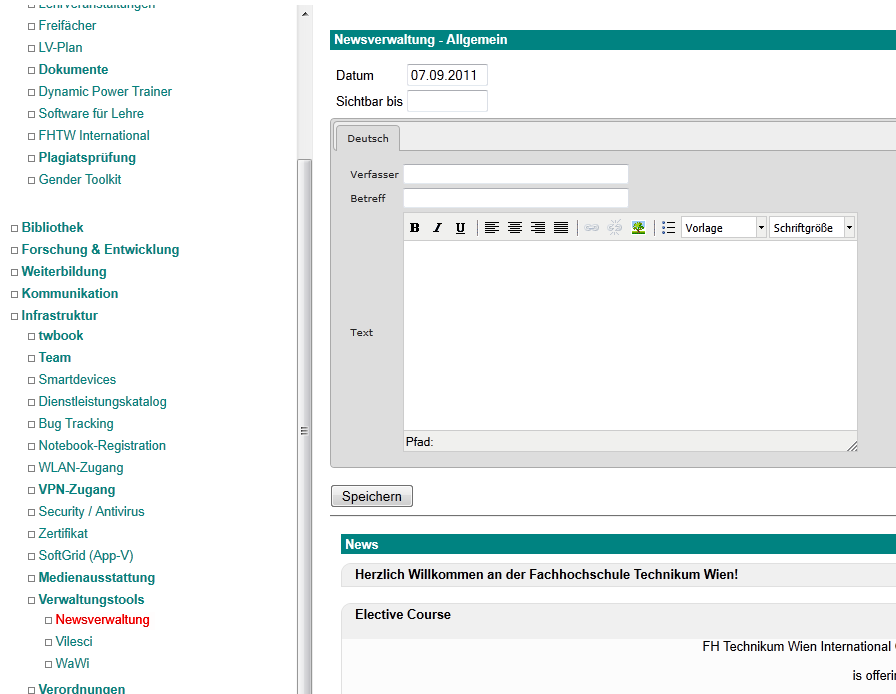
\includegraphics[width=0.70\textwidth]{CIS_Newsverwaltung_01.png}
	\caption{CIS General News Administration}
	\label{CIS_newsverwaltung01}
\end{figure}

		\begin{itemize}
			\item In the "'Date"' field, enter the date from which the news entry should be visible (default: today).
			\item In the field "'Visible to"', enter the date until when the news entry should be visible (max. 30 days). This field is optional, and if left blank the news entry will remain visible for 30 days.
			\item Enter the author name which will appear in the title line of the news entry.
			\item Enter a meaningful title for the article.
			\item Enter the text for the news entry and format it with the appropriate buttons. Holding your mouse over the different buttons will bring up an infotip that explains each button's function.
			You can adjust the size of the editing window by clicking and dragging the lower right corner of the window until it is the desired size.
			\item Finally, save the news entry by clicking on the "'Save"' button.
			\item You will find information on how to translate a news entry in the chapter \ref{uebersetzung_eines_neweintrags}.
		\end{itemize}
		
\subsection{How to Publish an OU Specific News Entry}
The news administration for the OU news can be found by clicking on the menu item "'Courses"' and then selecting the desired degree program.
Finally, click on "'Lecturer's Section"' and "'Pinboard Administration"'.

\begin{figure}
	\centering
	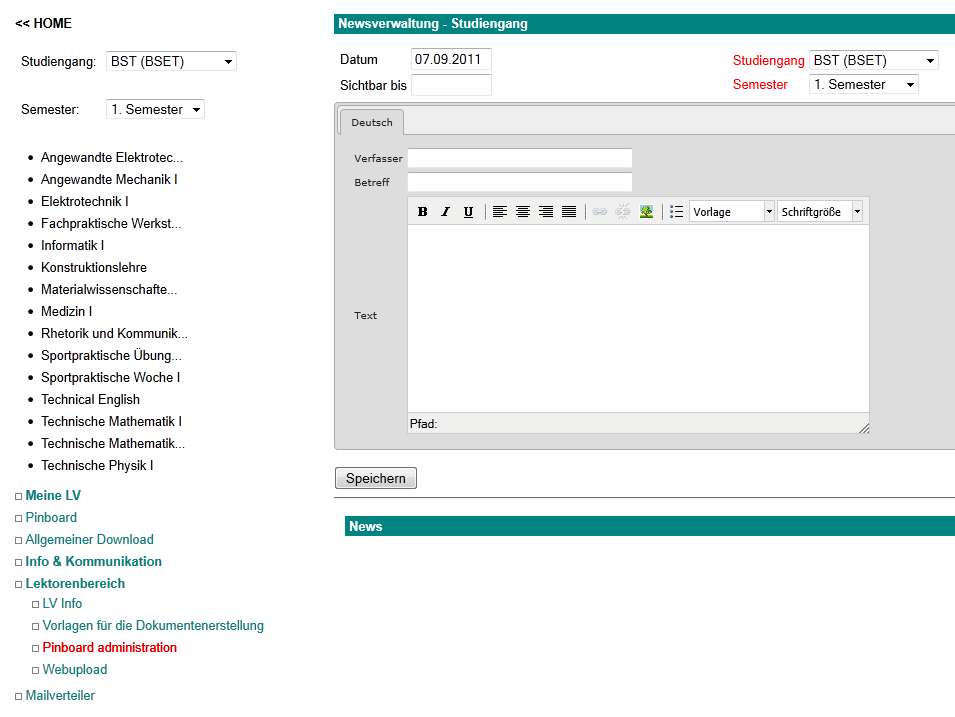
\includegraphics[width=0.70\textwidth]{CIS_Newsverwaltung_03.png}
	\caption{CIS News Administration for OU}
	\label{CIS_newsverwaltung03}
\end{figure}

Proceed with the news entry here the same as described in chapter \ref{allgemeinen_Newseintrag_erstellen} with the only difference being that you should select the relevant degree program and/or semester in the headline for those who should be able to view the news entry.

\subsection{How to Publish a Translation for a News Entry}
\label{uebersetzung_eines_neweintrags}
The Infrastructure will automatically send general news to the translator (does not apply for OU news) and will publish the translation as soon as it is available.
However, if you want to translate a news entry yourself or want to translate an OU news entry, please proceed as follows:
(also see chapter \ref{richtlinien_newseintraege} Guidelines for News Entries)
		\begin{itemize}
			\item After you have saved a news entry in the German language, a + symbol will appear next to the tab "'Deutsch"'.
				\begin{figure}
				\centering
				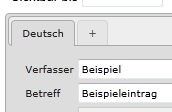
\includegraphics[width=0.30\textwidth]{CIS_Newsverwaltung_02.png}
				\end{figure}
			\item Click on "'+"' and select the desired language.
			\item Proceed with the news entry as described in Chapter \ref{allgemeinen_Newseintrag_erstellen}.
			\item Finally, save the news entry by clicking on the "'Save"' button.
		\end{itemize}
If the CIS page is now loaded in a different language, the news entry will now appear in the corresponding language if such a translation exists.
If there is no appropriate translation for a news entry in the German language, the news entry will be displayed in German.